
This example was conducted to show that, for an arbitrary isotope, the expected 
behavior is captured. In the case of real isotopes in a full simulation, the 
same model will be invoked with real parameters for each isotope. Thus, the 
this model agreement is representative in all cases.

In the parametric sensitivity analysis reported in \cite{huff_key_2012} it was 
shown that for solubility limits below a certain threshold, the dose releases 
were directly proportional to the solubility limit, indicating that the 
radionuclide concentration saturated the groundwater up to the solubility limit 
near the waste form.  For solubility limits above the threshold, however, 
further increase to the limit had no effect on the peak dose. This demonstrates 
the situation in which the solubility limit is so high that even complete 
dissolution of the waste inventory into the pore water is insufficient to reach 
the solubility limit.

In Figure \ref{fig:SolSumFactor}, it is clear that for 
solubility constants lower than a threshold, the transport regime is solubility 
limited and the relationship between peak annual dose and solubility limit is 
strong.  Above the threshold, the transport regime is inventory limited 
instead.

In the parametric analysis of \Cyder performance, it was shown that the 
solubility sensitivity behavior closely matched that of the \gls{GDSM} 
sensitivity behaviors. Specifically, in Figure \ref{fig:sol_result}, a sharp turnover 
is seen where the solubility limit exceeds the point at which it limits 
movement. For increased solubility limits, release remains constant.

\begin{figure}[ht]
\begin{center}
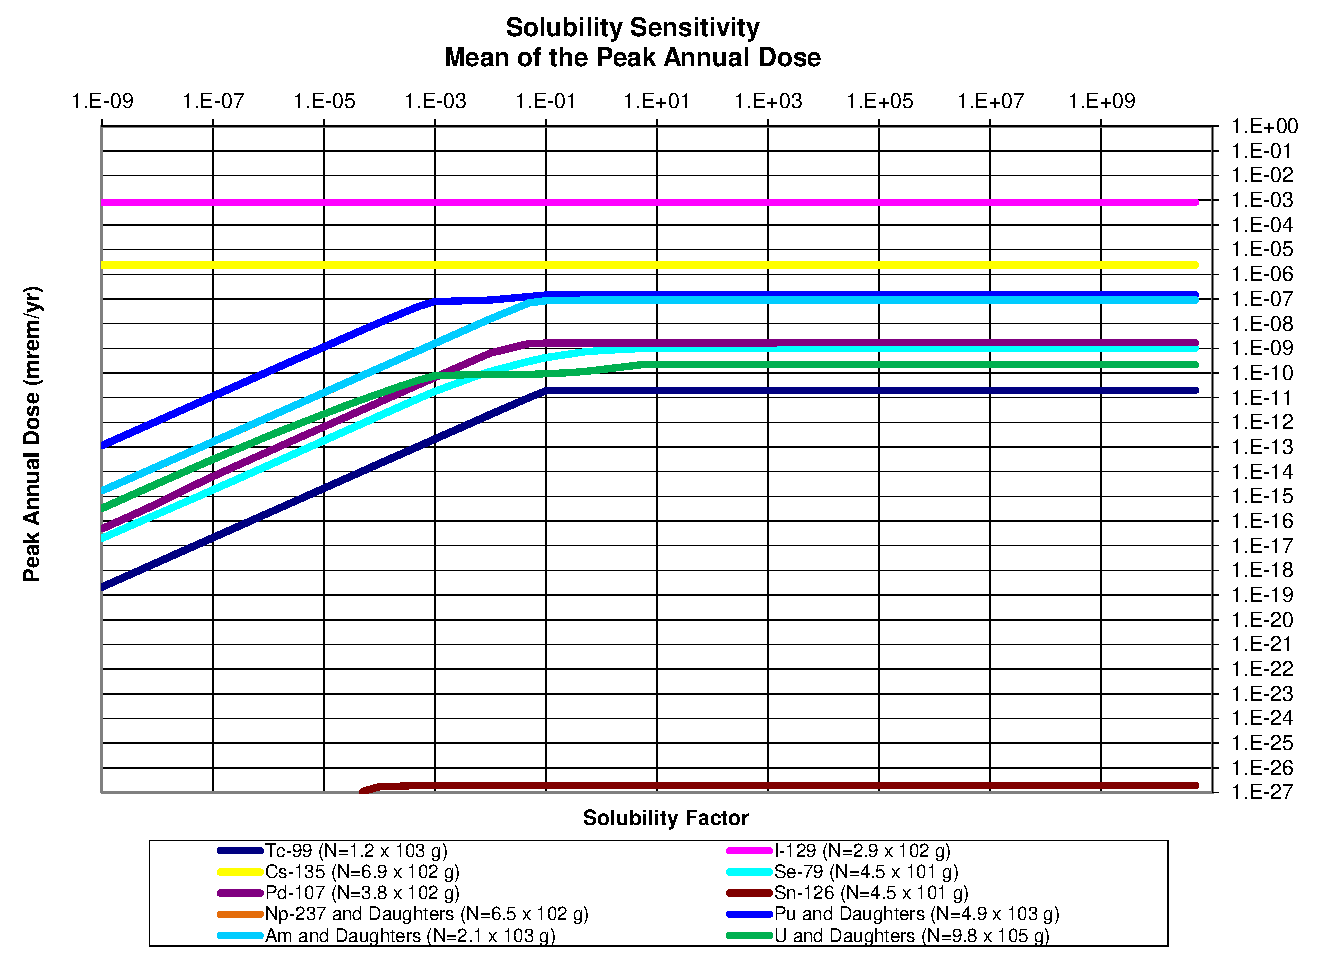
\includegraphics[width=0.7\linewidth]{./Solubility_Summary_SolFactor.eps}
\caption[Solubility factor sensitivity in GDSM Clay model]{Solubility factor sensitivity. The peak annual dose due to an inventory, 
$N$, of each isotope.}
\label{fig:SolSumFactor}
\end{center}
\end{figure}

%\begin{figure}[ht]
%\begin{center}
%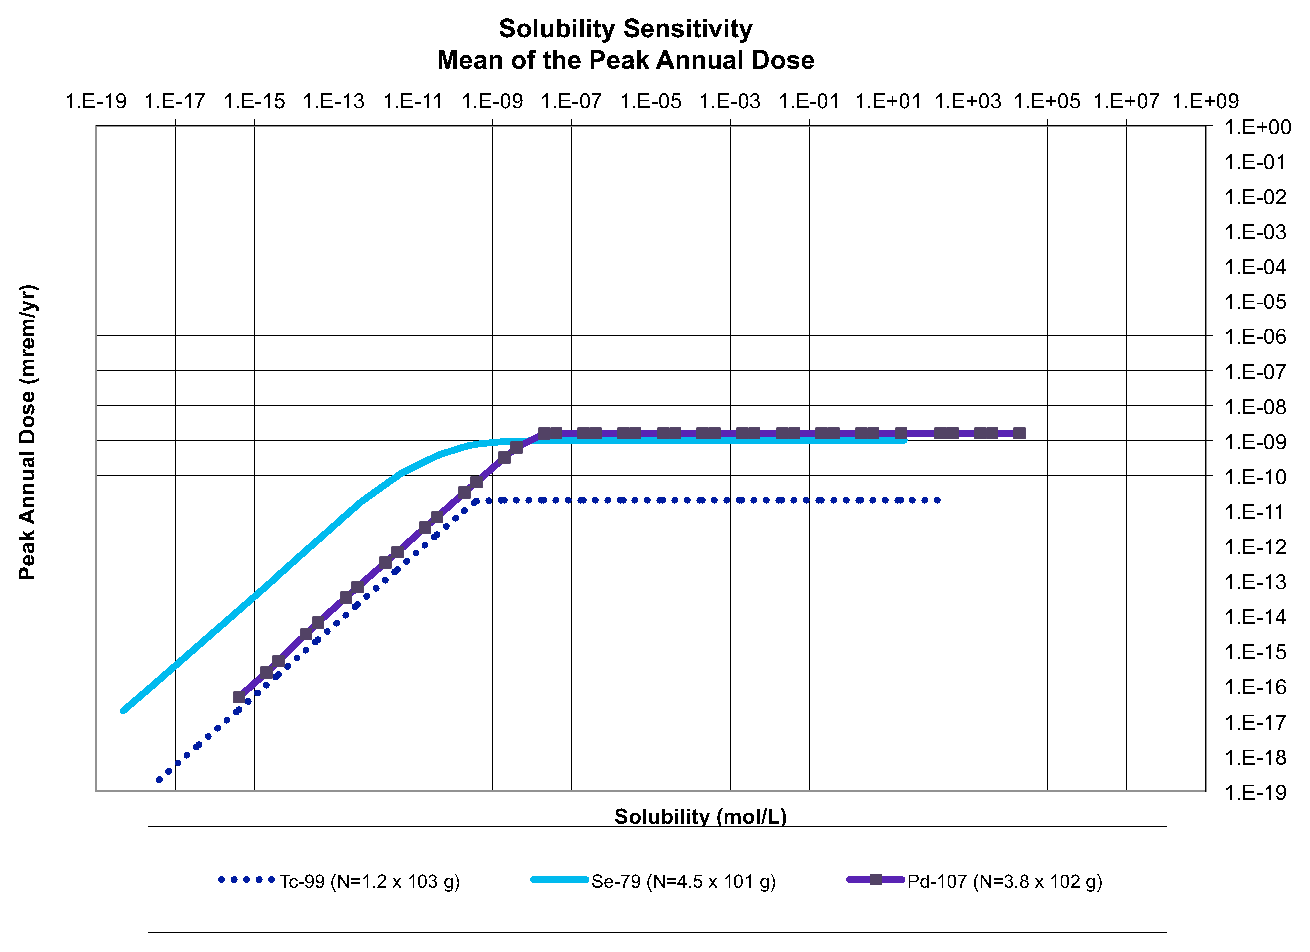
\includegraphics[width=0.7\linewidth]{./Solubility_Summary_Sol.eps}
%\caption[Solubility limit sensitivity in GDSM Clay model]{Solubility limit sensitivity. The peak annual dose due to an inventory, 
%$N$, of each isotope.}
%\label{fig:SolSum}
%\end{center}
%\end{figure}

\begin{figure}[htbp!]
\begin{center}
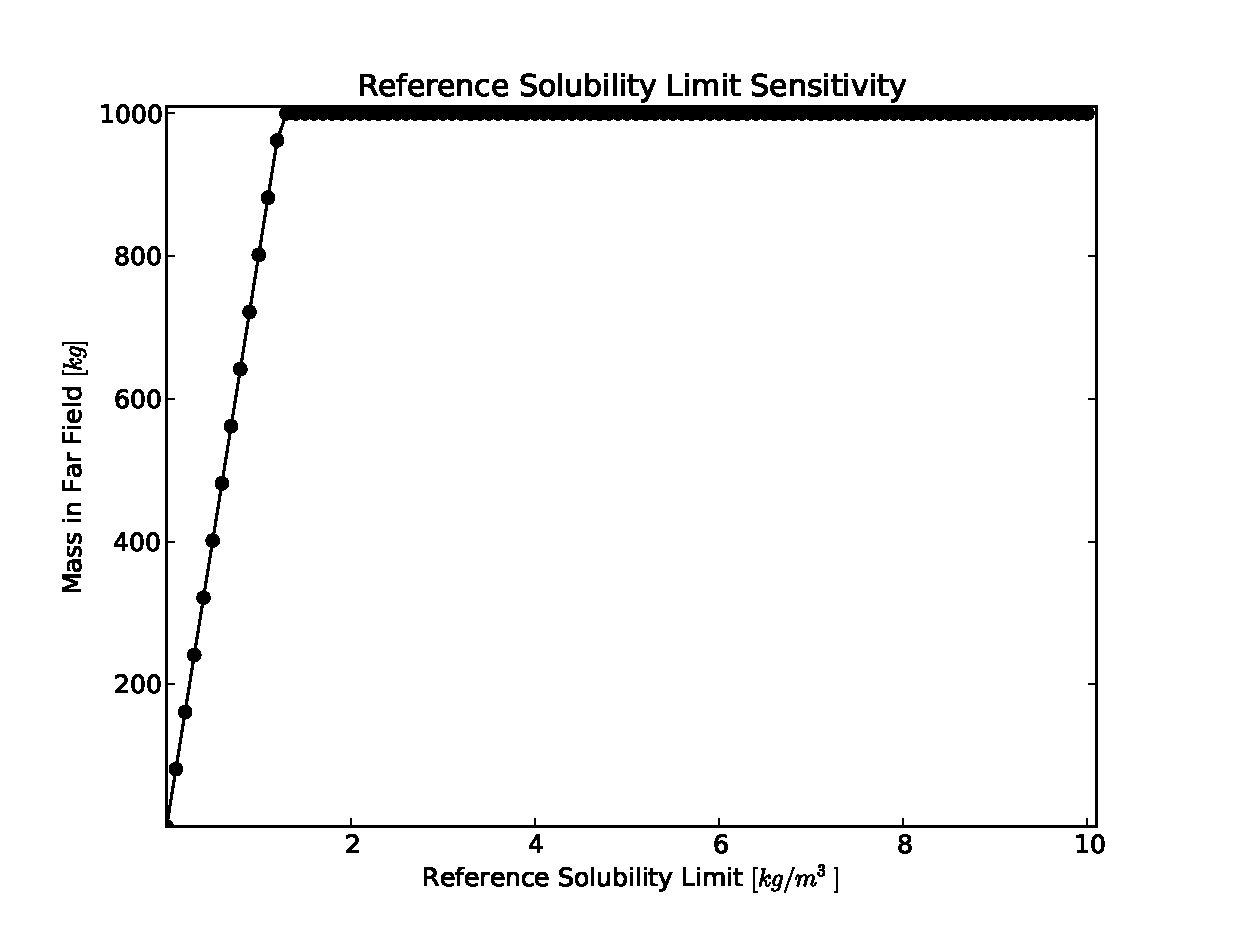
\includegraphics[width=0.7\linewidth]{./sol.eps}
\caption[Solubility Sensitivity in the Mixed Cell Model]{Sensitivity demonstration of solubility limitation in \Cyder for an arbitrary isotope assigned a variable solubility limit.}
\label{fig:sol_result}
\end{center}
\end{figure}
